\documentclass[12pt,a4paper]{article}

% Packages
\usepackage[utf8]{inputenc}
\usepackage[T1]{fontenc}
\usepackage[romanian]{babel}
\usepackage{geometry}
\geometry{margin=2.5cm}
\usepackage{graphicx}
\usepackage{hyperref}
\usepackage{listings}
\usepackage{xcolor}
\usepackage{booktabs}
\usepackage{amsmath,amsfonts,amssymb}
\usepackage{tcolorbox}
\usepackage{fancyhdr}
\usepackage{setspace}
\usepackage{caption}
\usepackage{subcaption}
\usepackage{enumitem}
\usepackage{array}
\usepackage{longtable}
\usepackage{float}

% Colors
\definecolor{codebg}{RGB}{248,248,248}
\definecolor{codeframe}{RGB}{200,200,200}
\definecolor{keyword}{RGB}{0,119,170}
\definecolor{string}{RGB}{163,21,21}
\definecolor{comment}{RGB}{0,128,0}
\definecolor{accentblue}{RGB}{41,128,185}

% Listings style
\lstset{
    language=SQL,
    basicstyle=\ttfamily\small,
    backgroundcolor=\color{codebg},
    frame=single,
    rulecolor=\color{codeframe},
    keywordstyle=\color{keyword}\bfseries,
    stringstyle=\color{string},
    commentstyle=\color{comment}\itshape,
    numbers=left,
    numberstyle=\tiny\color{gray},
    numbersep=8pt,
    breaklines=true,
    breakatwhitespace=true,
    showstringspaces=false,
    tabsize=2,
    captionpos=b,
    xleftmargin=15pt,
    framexleftmargin=15pt,
    aboveskip=10pt,
    belowskip=10pt
}

\lstdefinestyle{java}{
    language=Java,
    basicstyle=\ttfamily\small,
    backgroundcolor=\color{codebg},
    frame=single,
    rulecolor=\color{codeframe},
    keywordstyle=\color{keyword}\bfseries,
    stringstyle=\color{string},
    commentstyle=\color{comment}\itshape,
    numbers=left,
    numberstyle=\tiny\color{gray},
    numbersep=8pt,
    breaklines=true,
    tabsize=2,
    captionpos=b,
    xleftmargin=15pt,
    framexleftmargin=15pt
}

% Header/Footer
\pagestyle{fancy}
\fancyhf{}
\fancyhead[L]{\small Prognoza Meteo --- Proiect SGBD}
\fancyhead[R]{\small Negura Alexandru Teodor}
\fancyfoot[C]{\thepage}
\renewcommand{\headrulewidth}{0.4pt}

% tcolorbox styles
\tcbuselibrary{skins,breakable}
\newtcolorbox{infobox}[1][]{
    colback=blue!5!white,
    colframe=accentblue,
    fonttitle=\bfseries,
    title=#1,
    breakable
}

\newtcolorbox{algobox}[1][]{
    colback=gray!5!white,
    colframe=black!60,
    fonttitle=\bfseries,
    title=#1,
    breakable
}

\title{\Huge\textbf{Prognoza Meteo}\\[0.3cm]
\Large Aplicatie de prognoza meteo probabilistica cu algoritmi de Machine Learning in PostgreSQL\\[0.5cm]
\large Referat --- Proiect SGBD}
\author{
\textbf{Negura Alexandru Teodor}\\
Facultatea de Informatica\\
Universitatea ``Alexandru Ioan Cuza" din Iasi
}
\date{Anul universitar 2025--2026}

\begin{document}

\maketitle
\thispagestyle{empty}
\vfill
\begin{center}
\textit{Materie: Sisteme de Gestionare a Bazelor de Date (SGBD)}\\
\textit{Coordonator: Lect. Dr. Simona Varlan}
\end{center}
\newpage

% ========== CUPRINS ==========
\tableofcontents
\newpage

% ========== 1. INTRODUCERE ==========
\section{Introducere}

\subsection{Context si motivatie}

Prezenta lucrare descrie dezvoltarea unei aplicatii de prognoza meteo pentru orase din Europa, realizata in cadrul disciplinei \textbf{Sisteme de Gestionare a Bazelor de Date (SGBD)}. Proiectul imbina concepte avansate de modelare a datelor, programare in PL/pgSQL si implementarea unor algoritmi de Machine Learning direct la nivelul serverului de baze de date.

Spre deosebire de solutiile conventionale care externalizeaza logica predictiei catre biblioteci Python sau servicii cloud, abordarea noastra transfera \textbf{toti algoritmii de predictie} (vectorizare, clustering, lanturi Markov, Modele Markov Ascunse, simulare Monte Carlo) in interiorul PostgreSQL. Acest design are multiple avantaje:
\begin{itemize}[noitemsep]
    \item \textbf{Performanta}: predictiile sunt calculate direct acolo unde rezida datele, eliminand latenta de retea;
    \item \textbf{Tranzactionalitate}: actualizarile modelului si ale datelor sunt atomice;
    \item \textbf{Auditabilitate}: istoricul complet al parametrilor modelului este stocat in tabele relationale.
\end{itemize}

\subsection{Tehnologii utilizate}

\begin{table}[H]
\centering
\begin{tabular}{@{}ll@{}}
\toprule
\textbf{Strat} & \textbf{Tehnologie} \\
\midrule
Client desktop & Java 21 + JavaFX 23.0.2 \\
Conectivitate & JDBC (PostgreSQL 42.7.1) + HikariCP 5.1.0 \\
Server baze de date & PostgreSQL 16 (port 5433, Docker) \\
Procesare numerica & Apache Commons Math 3.6.1 \\
Serializare JSON & Jackson 2.16.1 \\
Testare & JUnit Jupiter 5.10.2 + Mockito 5.11.0 \\
Sursa date externa & Open-Meteo API (gratuit, fara cheie) \\
\bottomrule
\end{tabular}
\caption{Stack tehnologic al proiectului}
\end{table}

\subsection{Arhitectura generala}

Aplicatia urmeaza o arhitectura pe trei straturi:

\begin{enumerate}
    \item \textbf{Stratul de prezentare} --- interfata JavaFX cu 3 tab-uri: Dashboard unificat (prognoza curenta, evolutie, predictii, clasamente, anomalii), Harta interactiva (Europa cu 40 de tari si 66 de orase), si Management cont/comunitate.
    \item \textbf{Stratul de servicii} --- clase Java in pachetul \texttt{com.sgbd.service} care apeleaza proceduri stocate prin JDBC. Nu exista ORM; fiecare serviciu foloseste explicit \texttt{Connection}, \texttt{PreparedStatement} si \texttt{ResultSet} in blocuri \texttt{try-with-resources}.
    \item \textbf{Stratul de date} --- PostgreSQL cu 21 de tabele, 39 de proceduri stocate, 6 functii, 3 triggeri si 20+ indecsi specializati pentru algoritmii de Machine Learning.
\end{enumerate}

\begin{figure}[H]
\centering
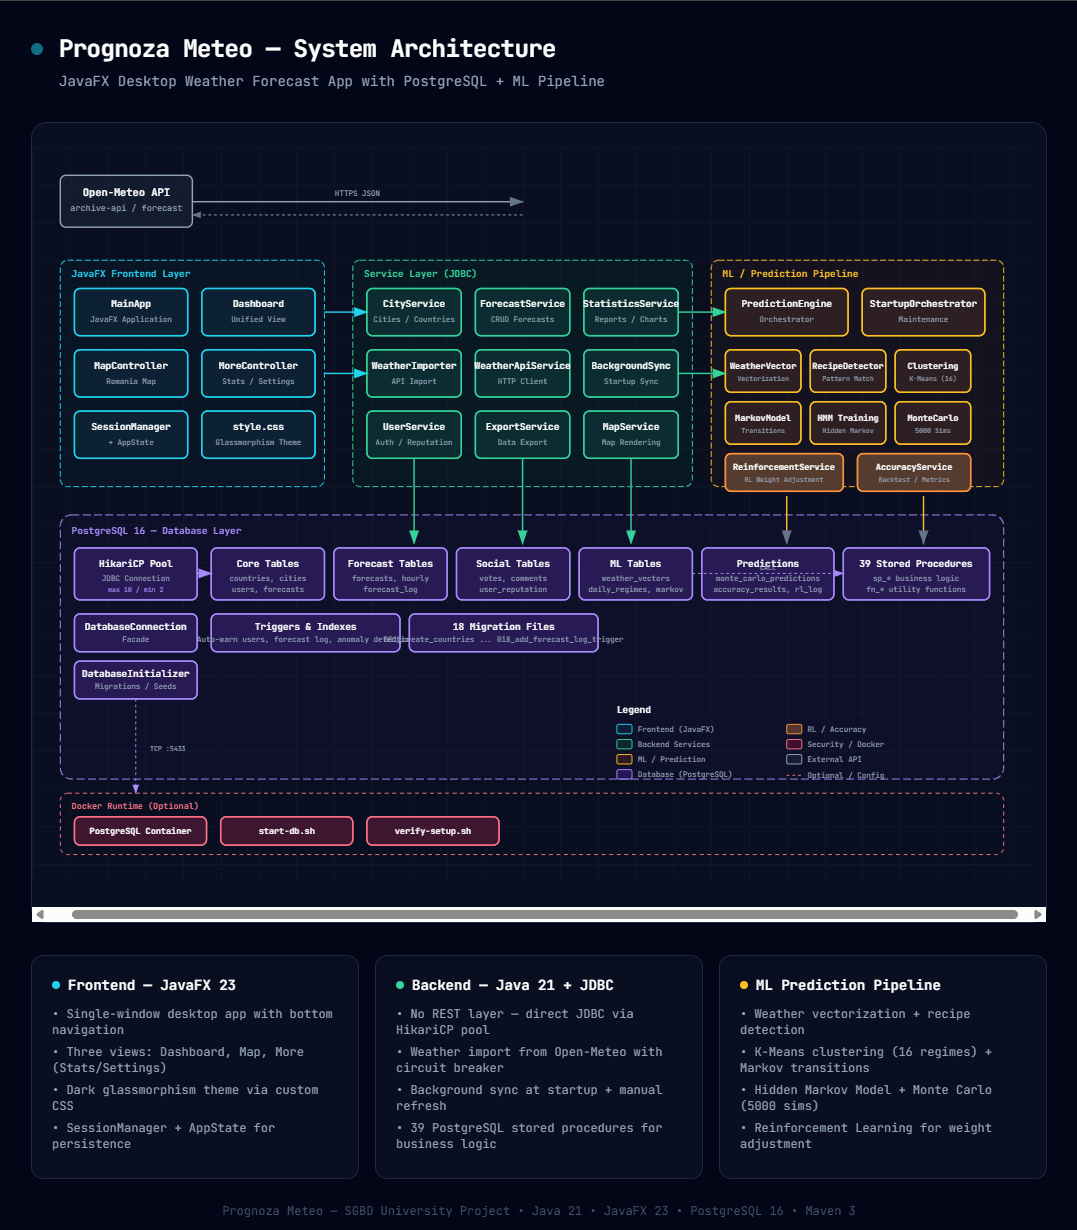
\includegraphics[width=0.60\textwidth]{screenshots/diagrama_arhitectura.png}
\caption{Diagrama arhitecturala a aplicatiei (din fisierul HTML interactiv)}
\label{fig:arhitectura}
\end{figure}

Diagrama arhitecturala interactiva (fisierul \texttt{prognoza-meteo-architecture.html} din repository) prezinta vizual cele trei straturi ale aplicatiei (JavaFX, Servicii Java/JDBC, PostgreSQL), procedurile stocate, fluxurile de date catre API-ul Open-Meteo si algoritmii de Machine Learning. Se recomanda includerea unui screenshot fullscreen al acestei diagrame in locul casetei de mai sus.

% ========== 2. CERINTE DE BUSINESS ==========
\section{Cerinte de business identificate}

Pe langa cerintele specificate in enuntul proiectului, am identificat si formalizat urmatoarele cerinte de business care ghideaza design-ul bazei de date si al algoritmilor:

\begin{infobox}[CB-1: Gestiunea entitatilor geografice]
Sistemul trebuie sa stocheze toate tarile si orasele din Europa cu coordonate geografice exacte (latitudine, longitudine). Fiecare oras apartine unei singure tari. Orasele marcate ca ``majore" (\texttt{is\_major = true}) sunt afisate pe harta interactiva.
\end{infobox}

\begin{infobox}[CB-2: Prognoze zilnice cu parametri completi]
Pentru fiecare pereche (oras, data) sistemul stocheaza: temperatura minima si maxima, viteza vantului, umiditatea relativa (0--100\%), indicele UV, pictograma meteo generata automat si un text de avertizare (optional). Toate campurile sunt obligatorii cu exceptia avertizarii.
\end{infobox}

\begin{infobox}[CB-3: Prognoze orare granulara]
Pentru analize de finete, sistemul stocheaza prognoze la nivel de ora (0--23) cu temperatura, umiditate, viteza vantului, probabilitatea de precipitatii si codul WMO al vremii.
\end{infobox}

\begin{infobox}[CB-4: Generarea automata a pictogramelor]
Pictograma nu este stocata static, ci este generata dinamic prin procedura \texttt{sp\_generate\_icon} pe baza unei logici fuzzy care combina temperatura, umiditatea, precipitatiile, viteza vantului si indicele UV.
\end{infobox}

\begin{infobox}[CB-5: Avertizari meteo contextuale]
Sistemul detecteaza automat situatii periculoase (canicula, furtuna, ceata densa) si genereaza avertizari cu recomandari specifice (``Stati acasa", ``Luati umbrela").
\end{infobox}

\begin{infobox}[CB-6: Feedback comunitar si reputatie]
Utilizatorii autentificati pot vota acuratetea unei prognoze (corecta/eronata) si pot adauga comentarii. Reputatia fiecarui utilizator este recalculata automat prin trigger la fiecare vot nou, utilizand o formula logaritmica ponderata.
\end{infobox}

\begin{infobox}[CB-7: Predictii probabilistice pe 10 zile]
Sistemul genereaza predictii pentru urmatoarele 10 zile sub forma de benzi de incredere (P10, P50, P90) folosind simulare Monte Carlo cu 5000 de traiectorii. Fiecare traiectorie este construita prin tranzitii de regimuri Markov de ordin 2, ajustate cu climatologie sezoniera.
\end{infobox}

\begin{infobox}[CB-8: Detectie anomalii si prognoze contestate]
Sistemul identifica automat prognozele care deviaza statistic de la climatologia locala (regula celor $2\sigma$) si le marcheaza ca anomalii. De asemenea, identifica prognozele cu erori mari fata de realitate (comparand cu datele Open-Meteo).
\end{infobox}

\begin{infobox}[CB-9: Clasamente si similaritati]
Orasele pot fi clasate dupa 6 criterii (cel mai cald, cel mai frig, cel mai vantos etc.) si pot fi grupate in functie de similaritatea euclidiana a profilurilor meteorologice pe o perioada data.
\end{infobox}

\begin{infobox}[CB-10: Avertizare automata a utilizatorilor]
La detectarea unui eveniment extrem, procedura stocata \texttt{sp\_auto\_warn\_users} notifica automat toti utilizatorii care au interactionat recent cu prognozele din zona afectata.
\end{infobox}

% ========== 3. NORMALIZAREA BAZEI DE DATE ==========
\section{Normalizarea bazei de date}

\subsection{Relatia universala initiala}

Pornim de la o singura relatie universala care incapsuleaza toate datele meteorologice:

\begin{align*}
R(\underline{\text{country\_name}}, &\text{ city\_name}, \text{ date}, \text{ temp\_min}, \text{ temp\_max}, \text{ wind\_speed}, \\
&\text{ humidity}, \text{ uv\_index}, \text{ icon\_type}, \text{ warning\_text}, \\
&\text{ username}, \text{ vote\_value}, \text{ comment\_text})
\end{align*}

\textbf{Cheie candidat}: $\{\text{country\_name}, \text{ city\_name}, \text{ date}, \text{ username}, \text{ vote\_timestamp}\}$

\subsection{Analiza dependentelor functionale}

Din cerintele de business extragem urmatoarele dependente functionale:

\begin{align*}
\text{country\_name} &\rightarrow \text{country\_code, continent} \\
\text{city\_name, country\_name} &\rightarrow \text{latitude, longitude, population} \\
\text{city\_name, date} &\rightarrow \text{temp\_min, temp\_max, wind\_speed, humidity, uv\_index, icon\_type, warning\_text} \\
\text{username} &\rightarrow \text{password\_hash, email, reputation} \\
\text{username, city\_name, date} &\rightarrow \text{vote\_value} \\
\text{username, city\_name, date, comment\_timestamp} &\rightarrow \text{comment\_text}
\end{align*}

\subsection{Procesul de normalizare}

\subsubsection{1NF --- Forma normala 1}

Relatia $R$ este atomica la nivel de celula (fiecare atribut contine o singura valoare). Nu exista atribute multivaluate sau compuse. Cu toate acestea, sufera de anomalii de inserare, stergere si actualizare:
\begin{itemize}[noitemsep]
    \item \textbf{Anomalie de inserare}: nu putem adauga o tara noua fara sa avem cel putin un oras cu prognoza;
    \item \textbf{Anomalie de stergere}: stergand singura prognoza a unui oras, pierdem si datele geografice ale orasului;
    \item \textbf{Anomalie de actualizare}: schimbarea codului ISO al unei tari necesita modificari in toate tuplele care o referentiaza.
\end{itemize}

\subsubsection{2NF --- Eliminarea dependentelor partiale}

Cheia primara este compusa. Observam dependente partiale:
\begin{itemize}
    \item $\text{country\_name} \rightarrow \text{country\_code}$ (dependenta de o parte a cheii);
    \item $\text{city\_name, country\_name} \rightarrow \text{latitude, longitude}$ (similar).
\end{itemize}

\textbf{Descompunere in 2NF}:
\begin{align*}
R_1(\underline{\text{country\_name}}, \text{ country\_code}, \text{ continent}) \\
R_2(\underline{\text{city\_name}}, \text{ country\_name}, \text{ latitude}, \text{ longitude}, \text{ population}) \\
R_3(\underline{\text{city\_name}, \text{ date}}, \text{ temp\_min}, \text{ temp\_max}, \dots, \text{ warning\_text}) \\
R_4(\underline{\text{username}}, \text{ password\_hash}, \text{ email}, \text{ reputation}) \\
R_5(\underline{\text{username}, \text{ city\_name}, \text{ date}}, \text{ vote\_value}) \\
R_6(\underline{\text{username}, \text{ city\_name}, \text{ date}, \text{ comment\_ts}}, \text{ comment\_text})
\end{align*}

\subsubsection{3NF --- Eliminarea dependentelor tranzitive}

Verificam fiecare relatie:
\begin{itemize}
    \item $R_1$: toate atributele non-cheie depind direct de \texttt{country\_name}. \textbf{Este in 3NF}.
    \item $R_2$: toate atributele depind direct de cheia $\{\text{city\_name}\}$. \textbf{Este in 3NF}.
    \item $R_3$: nu exista dependente tranzitive intre atributele non-cheie. \textbf{Este in 3NF}.
    \item $R_4$: nu exista dependente tranzitive. \textbf{Este in 3NF}.
    \item $R_5, R_6$: relatii asociative cu toate atributele in cheie sau dependente direct de cheie. \textbf{Sunt in 3NF}.
\end{itemize}

\subsubsection{BCNF --- Forma normala Boyce-Codd}

O relatie este in BCNF daca pentru fiecare DF $X \rightarrow Y$, $X$ este supercheie.
\begin{itemize}
    \item $R_1$: \texttt{country\_name} este PK $\Rightarrow$ \textbf{BCNF}.
    \item $R_2$: \texttt{city\_name} este PK $\Rightarrow$ \textbf{BCNF}.
    \item $R_3$: cheia este $\{\text{city\_name}, \text{date}\}$. Toate DF au determinantul cheie $\Rightarrow$ \textbf{BCNF}.
    \item $R_4$: \texttt{username} este PK $\Rightarrow$ \textbf{BCNF}.
    \item $R_5, R_6$: cheile sunt compuse si toate DF sunt cheie $\rightarrow$ atribut $\Rightarrow$ \textbf{BCNF}.
\end{itemize}

\subsection{Extensia pentru algoritmii de Machine Learning}

Algoritmii de Machine Learning introduc tabele suplimentare care, prin design, sunt deja normalizate:

\begin{itemize}
    \item \texttt{weather\_vectors}: cheia este compusa $(\text{city\_id}, \text{forecast\_date})$. Vectorul de 25 de dimensiuni este un atribut compus care reprezinta o singura valoare (vectorul caracteristic al zilei), deci respecta 1NF.
    \item \texttt{markov\_transitions}: cheia implicita este $(\text{climate\_zone}, \text{season}, \text{r\_prev}, \text{r\_curr}, \text{r\_next})$. Probabilitatea depinde functional de intreaga cheie $\Rightarrow$ \textbf{BCNF}.
    \item \texttt{monte\_carlo\_predictions}: cheia compusa $(\text{city\_id}, \text{forecast\_date}, \text{horizon\_day})$. Toate percentilele depind de aceasta cheie $\Rightarrow$ \textbf{BCNF}.
\end{itemize}

\begin{table}[H]
\centering\small\setlength{\tabcolsep}{4pt}
\begin{tabular}{@{}llccc@{}}
\toprule
\textbf{Tabela} & \textbf{PK/FK} & \textbf{1NF} & \textbf{2NF} & \textbf{BCNF} \\
\midrule
\texttt{countries} & id & Da & Da & Da \\
\texttt{cities} & id $\rightarrow$ countries & Da & Da & Da \\
\texttt{forecasts} & id $\rightarrow$ cities & Da & Da & Da \\
\texttt{hourly\_forecasts} & id $\rightarrow$ cities & Da & Da & Da \\
\texttt{users} & id & Da & Da & Da \\
\texttt{votes} & id $\rightarrow$ users, forecasts & Da & Da & Da \\
\texttt{comments} & id $\rightarrow$ users, forecasts, self & Da & Da & Da \\
\texttt{weather\_vectors} & id $\rightarrow$ cities & Da & Da & Da \\
\texttt{weather\_regimes} & id $\rightarrow$ cities & Da & Da & Da \\
\texttt{daily\_regimes} & id $\rightarrow$ cities & Da & Da & Da \\
\texttt{markov\_transitions} & id & Da & Da & Da \\
\texttt{hidden\_states} & id $\rightarrow$ cities & Da & Da & Da \\
\texttt{hidden\_transitions} & id $\rightarrow$ cities & Da & Da & Da \\
\texttt{monte\_carlo\_pred} & id $\rightarrow$ cities & Da & Da & Da \\
\texttt{seasonal\_climatology} & id $\rightarrow$ cities & Da & Da & Da \\
\texttt{prediction\_accuracy} & id $\rightarrow$ cities & Da & Da & Da \\
\texttt{forecast\_log} & id $\rightarrow$ forecasts & Da & Da & Da \\
\bottomrule
\end{tabular}
\caption{Verificarea formelor normale (toate tabelele sunt in BCNF)}
\end{table}

\vspace{0.8cm}

% ========== 4. DIAGRAMA E/A ==========
\section{Diagrama entitate-asociere (UML)}

Diagrama E/A a fost realizata conform standardului UML pentru diagrame de clase, adaptat pentru modelul entitate-relatie. Fiecare clasa reprezinta o entitate, iar asocierile sunt etichetate cu multiplicitatea corespunzatoare.

\subsection{Entitati identificate}

\begin{enumerate}
    \item \textbf{countries} --- entitate independenta care stocheaza tarile Europei.
    \item \textbf{cities} --- entitate dependenta de \texttt{countries}; fiecare oras apartine exact unei tari.
    \item \textbf{forecasts} --- entitate centrala; fiecare prognoza apartine unui oras si unei date.
    \item \textbf{hourly\_forecasts} --- specializare granulara a prognozei (nivel de ora).
    \item \textbf{users} --- entitate independenta pentru gestiunea conturilor.
    \item \textbf{votes} --- entitate asociativa intre \texttt{users} si \texttt{forecasts}.
    \item \textbf{comments} --- entitate asociativa cu auto-referinta (raspunsuri la comentarii).
    \item \textbf{weather\_vectors} --- entitate care stocheaza reprezentarea vectoriala a zilei.
    \item \textbf{weather\_regimes} --- entitate care defineste regimurile meteorologice (clustere).
    \item \textbf{daily\_regimes} --- entitate asociativa care leaga fiecare zi de regimul sau.
    \item \textbf{markov\_transitions} --- entitate care stocheaza tensorul de tranzitii Markov.
    \item \textbf{hidden\_states} / \textbf{hidden\_transitions} --- entitati HMM.
    \item \textbf{monte\_carlo\_predictions} --- entitate pentru rezultatele simularii.
    \item \textbf{seasonal\_climatology} --- entitate pentru climatologia sezoniera.
    \item \textbf{prediction\_accuracy} --- entitate pentru metrici de acuratete.
    \item \textbf{forecast\_log} --- entitate de audit.
\end{enumerate}

\subsection{Asocieri si multiplicitati}

\begin{table}[H]
\centering\small\setlength{\tabcolsep}{5pt}
\begin{tabular}{@{}llcc@{}}
\toprule
\textbf{Sursa} & \textbf{Tinta} & \textbf{Tip} & \textbf{Mult.} \\
\midrule
\texttt{countries} & \texttt{cities} & compozitie & 1 : 0..* \\
\texttt{cities} & \texttt{forecasts} & compozitie & 1 : 0..* \\
\texttt{cities} & \texttt{hourly\_fc} & compozitie & 1 : 0..* \\
\texttt{cities} & \texttt{weather\_vec} & compozitie & 1 : 0..* \\
\texttt{cities} & \texttt{daily\_reg} & compozitie & 1 : 0..* \\
\texttt{cities} & \texttt{hidden\_st} & compozitie & 1 : 0..* \\
\texttt{cities} & \texttt{mc\_pred} & compozitie & 1 : 0..* \\
\texttt{forecasts} & \texttt{votes} & agregare & 1 : 0..* \\
\texttt{forecasts} & \texttt{comments} & agregare & 1 : 0..* \\
\texttt{forecasts} & \texttt{forecast\_log} & agregare & 1 : 0..* \\
\texttt{users} & \texttt{votes} & asociere & 1 : 0..* \\
\texttt{users} & \texttt{comments} & asociere & 1 : 0..* \\
\texttt{comments} & \texttt{comments} & auto-ref & 1 : 0..* \\
\bottomrule
\end{tabular}
\caption{Asocieri intre entitati (abrevieri: fc=forecasts, vec=vectors, reg=regimes, st=states, mc=monte\_carlo)}
\end{table}

\subsection{Justificarea cheilor primare si straine}

\begin{itemize}
    \item \texttt{countries.id}: aleasa ca \texttt{SERIAL} (auto-increment) pentru a permite inserarea automata fara specificarea explicita a ID-ului. Alternativa \texttt{code} (ISO) ar fi fost naturala, dar codurile ISO pot suferi modificari rare in timp (ex. Yugoslavia). Cheia surrogate este mai stabila.
    \item \texttt{cities.country\_id}: cheie straina catre \texttt{countries}. Impune integritatea referentiala: nu putem sterge o tara care are orase asociate (comportament \texttt{ON DELETE RESTRICT}).
    \item \texttt{forecasts.city\_id + date}: constrangerea \texttt{UNIQUE} asigura o singura prognoza pe zi pentru fiecare oras. Cheia primara \texttt{id} este surrogate pentru eficienta indecsilor.
    \item \texttt{hourly\_forecasts.city\_id + forecast\_date + hour}: constrangere \texttt{UNIQUE} care garanteaza o singura inregistrare orara per oras-data-ora.
    \item \texttt{comments.parent\_comment\_id}: cheie straina auto-referentiala care permite ierarhii de comentarii (raspunsuri). Este nullable pentru comentariile de nivel 0.
\end{itemize}

\subsection{Tipuri de constrangeri}

Conform teoriei bazelor de date, exista 5 tipuri de constrangeri. Iata cum sunt implementate in proiect:

\begin{enumerate}
    \item \textbf{Constrangeri de domeniu (Domain Constraints)}: \texttt{CHECK(humidity BETWEEN 0 AND 100)}, \texttt{CHECK(hour BETWEEN 0 AND 23)}, \texttt{CHECK(latitude BETWEEN -90 AND 90)}.
    \item \textbf{Constrangeri de entitate (Entity Integrity)}: toate tabelele au \texttt{PRIMARY KEY} care garanteaza unicitatea si non-nullitatea identificatorului.
    \item \textbf{Constrangeri referentiale (Referential Integrity)}: 18 chei straine cu \texttt{REFERENCES} care garanteaza ca valorile din coloana copil exista in tabela parinte.
    \item \textbf{Constrangeri de unicitate (Key Constraints)}: \texttt{UNIQUE(name, country\_id)} pe \texttt{cities}, \texttt{UNIQUE(username)} pe \texttt{users}, \texttt{UNIQUE(city\_id, forecast\_date, hour)} pe \texttt{hourly\_forecasts}.
    \item \textbf{Constrangeri de verificare (Check Constraints)}: \texttt{CHECK(temp\_min <= temp\_max)} pe \texttt{forecasts}, \texttt{CHECK(precipitation\_probability BETWEEN 0 AND 100)} pe \texttt{hourly\_forecasts}.
\end{enumerate}

\begin{figure}[H]
\centering
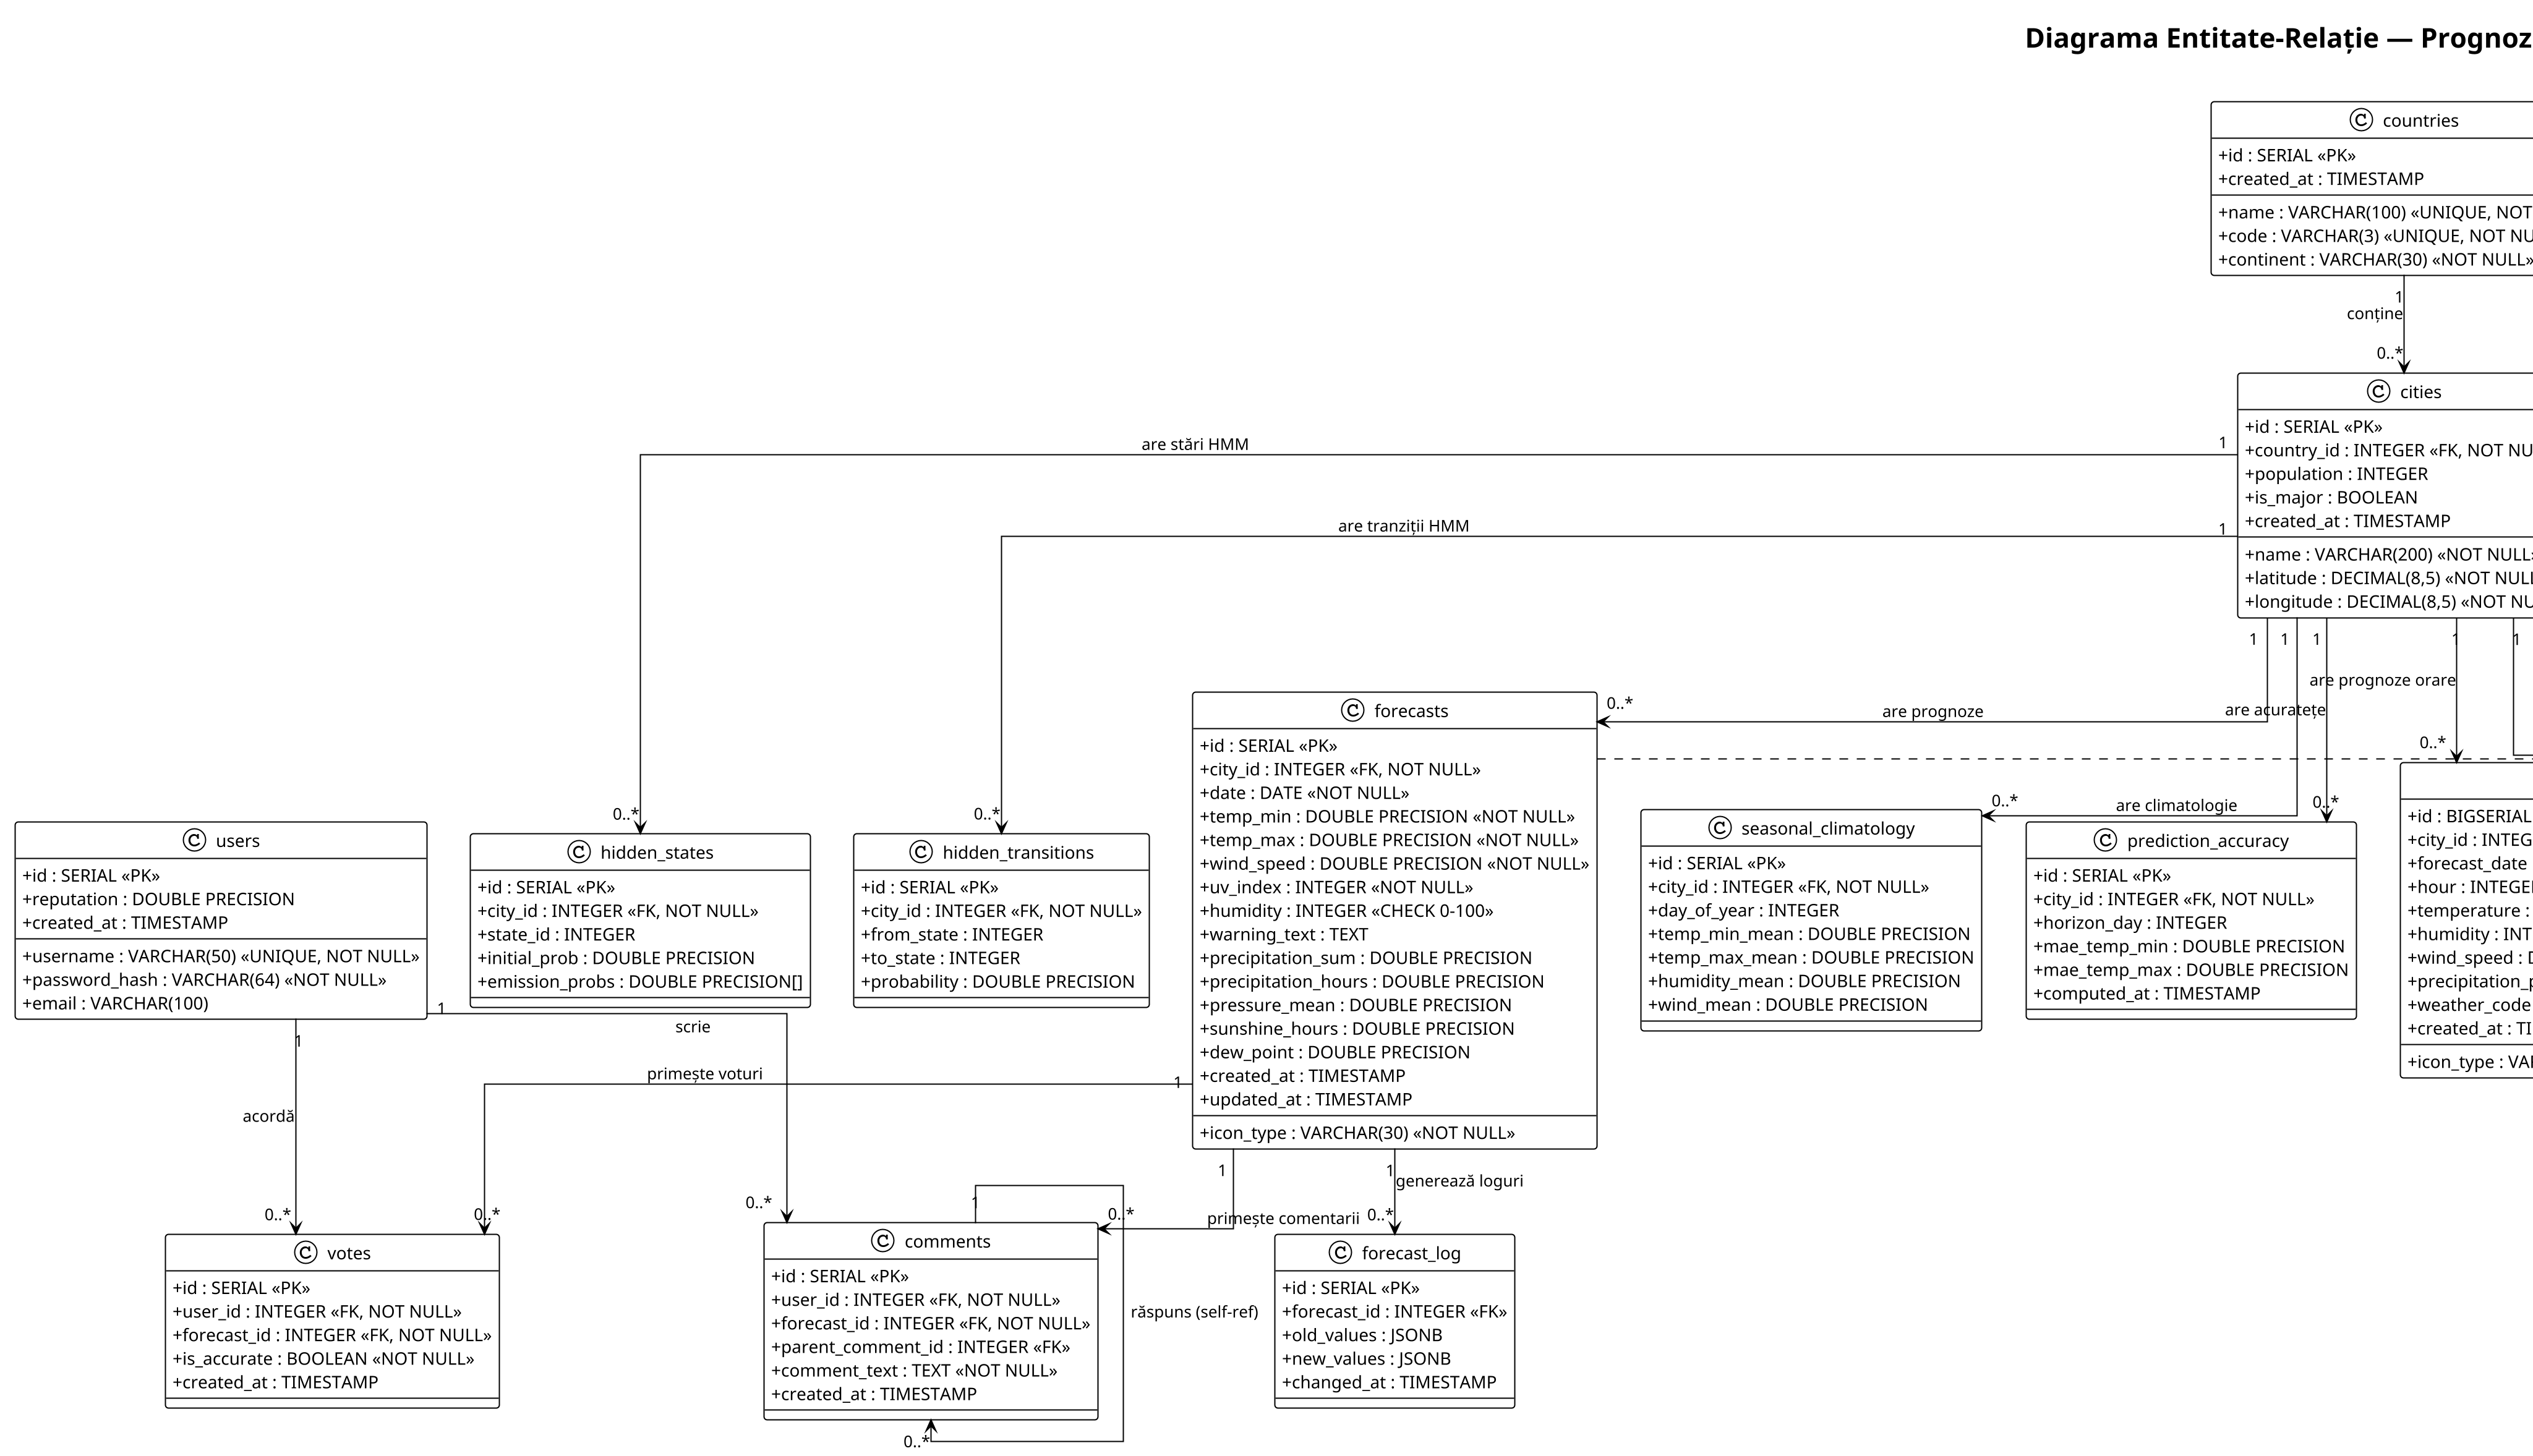
\includegraphics[width=0.60\textwidth]{screenshots/er_diagram.png}
\caption{Diagrama entitate-relatie (UML) a bazei de date}
\label{fig:er}
\end{figure}

\vspace{0.8cm}

% ========== 5. SCRIPT DE CREARE TABELE ==========
\section{Script de creare a tabelelor}

Migrarile sunt organizate in fisiere numerotate in directorul \texttt{db/migrations/}. Fiecare fisier este atomic si idempotent (foloseste \texttt{IF NOT EXISTS}). Prezentam mai jos cele mai importante scripturi cu explicatii detaliate.

\subsection{Migrarea 001: Tari}

\begin{lstlisting}[caption={Crearea tabelei \texttt{countries}}]
CREATE TABLE IF NOT EXISTS countries (
    id SERIAL PRIMARY KEY,
    name VARCHAR(100) NOT NULL UNIQUE,
    code VARCHAR(3) NOT NULL UNIQUE,
    continent VARCHAR(30) NOT NULL,
    created_at TIMESTAMP NOT NULL DEFAULT CURRENT_TIMESTAMP
);
\end{lstlisting}

\textbf{Explicatii}:
\begin{itemize}[noitemsep]
    \item \texttt{id SERIAL} creeaza automat o secventa \texttt{countries\_id\_seq} pentru auto-increment;
    \item \texttt{UNIQUE} pe \texttt{name} si \texttt{code} previne duplicarea tarilor;
    \item Nu exista FK deoarece este entitatea radacina.
\end{itemize}

\subsection{Migrarea 002: Orase}

\begin{lstlisting}[caption={Crearea tabelei \texttt{cities} cu FK si constrangeri}]
CREATE TABLE IF NOT EXISTS cities (
    id SERIAL PRIMARY KEY,
    name VARCHAR(200) NOT NULL,
    country_id INTEGER NOT NULL REFERENCES countries(id),
    latitude DECIMAL(8,5) NOT NULL,
    longitude DECIMAL(8,5) NOT NULL,
    population INTEGER,
    timezone VARCHAR(50),
    is_major BOOLEAN NOT NULL DEFAULT FALSE,
    created_at TIMESTAMP NOT NULL DEFAULT CURRENT_TIMESTAMP,
    UNIQUE(name, country_id),
    CHECK(latitude BETWEEN -90 AND 90),
    CHECK(longitude BETWEEN -180 AND 180)
);
\end{lstlisting}

\textbf{Explicatii}:
\begin{itemize}[noitemsep]
    \item \texttt{REFERENCES countries(id)} este cheia straina care leaga fiecare oras de tara sa;
    \item \texttt{UNIQUE(name, country\_id)} permite existenta unor orase cu acelasi nume in tari diferite (ex. ``Newcastle" in UK si Australia), dar interzice duplicatele in aceeasi tara;
    \item Constrangerile \texttt{CHECK} valideaza domeniul coordonatelor geografice.
\end{itemize}

\subsection{Migrarea 003: Prognoze zilnice}

\begin{lstlisting}[caption={Crearea tabelei \texttt{forecasts}}]
CREATE TABLE IF NOT EXISTS forecasts (
    id SERIAL PRIMARY KEY,
    city_id INTEGER NOT NULL REFERENCES cities(id),
    date DATE NOT NULL,
    temp_min DOUBLE PRECISION NOT NULL,
    temp_max DOUBLE PRECISION NOT NULL,
    wind_speed DOUBLE PRECISION NOT NULL,
    icon_type VARCHAR(30) NOT NULL,
    uv_index INTEGER NOT NULL,
    humidity INTEGER NOT NULL CHECK (humidity BETWEEN 0 AND 100),
    warning_text TEXT,
    created_at TIMESTAMP NOT NULL DEFAULT CURRENT_TIMESTAMP,
    updated_at TIMESTAMP NOT NULL DEFAULT CURRENT_TIMESTAMP,
    UNIQUE(city_id, date)
);
\end{lstlisting}

\textbf{Explicatii}:
\begin{itemize}[noitemsep]
    \item \texttt{UNIQUE(city\_id, date)} modeleaza constrangerea de business ``o singura prognoza pe zi per oras";
    \item \texttt{CHECK (humidity BETWEEN 0 AND 100)} valideaza ca umiditatea este un procent valid;
    \item \texttt{updated\_at} este mentinut automat de trigger-ul \texttt{trg\_forecasts\_updated\_at}.
\end{itemize}

\subsection{Migrarea 015: Triggeri}

\begin{lstlisting}[caption={Trigger pentru actualizarea automata a timestamp-ului}]
CREATE OR REPLACE FUNCTION fn_update_timestamp()
RETURNS TRIGGER AS $$
BEGIN
    NEW.updated_at = CURRENT_TIMESTAMP;
    RETURN NEW;
END;
$$ LANGUAGE plpgsql;

CREATE TRIGGER trg_forecasts_updated_at
BEFORE UPDATE ON forecasts
FOR EACH ROW
EXECUTE FUNCTION fn_update_timestamp();
\end{lstlisting}

\textbf{Explicatii}:
\begin{itemize}[noitemsep]
    \item Functia \texttt{fn\_update\_timestamp} este reutilizabila pentru orice tabel care are coloana \texttt{updated\_at};
    \item Trigger-ul \texttt{BEFORE UPDATE} se declanseaza inainte ca modificarea sa fie scrisa, astfel incat valoarea noua a timestamp-ului este inclusa in UPDATE.
\end{itemize}

\begin{lstlisting}[caption={Trigger pentru recalcularea reputatiei la vot}]
CREATE OR REPLACE FUNCTION fn_update_reputation()
RETURNS TRIGGER AS $$
BEGIN
    UPDATE users
    SET reputation = (
        SELECT COALESCE(AVG(CASE WHEN v.is_accurate THEN 1.0 ELSE 0.0 END), 0.5)
        FROM votes v
        WHERE v.user_id = NEW.user_id
    ) * LN(1 + (
        SELECT COUNT(*) FROM comments WHERE user_id = NEW.user_id
    ) + 1)
    WHERE id = NEW.user_id;
    RETURN NEW;
END;
$$ LANGUAGE plpgsql;

CREATE TRIGGER trg_update_reputation_on_vote
AFTER INSERT ON votes
FOR EACH ROW
EXECUTE FUNCTION fn_update_reputation();
\end{lstlisting}

\textbf{Explicatii}:
\begin{itemize}[noitemsep]
    \item Trigger-ul \texttt{AFTER INSERT} asigura ca votul este deja persistat inainte de recalculare;
    \item Formula combina acuratetea voturilor (medie binara) cu un factor logaritmic de activitate (numarul de comentarii);
    \item \texttt{COALESCE} gestioneaza cazul in care utilizatorul nu are voturi (reputatie default 0.5).
\end{itemize}

\subsection{Migrarea 018: Trigger de audit}

\begin{lstlisting}[caption={Trigger pentru logarea modificarilor de prognoze}]
CREATE OR REPLACE FUNCTION fn_log_forecast_change()
RETURNS TRIGGER AS $$
BEGIN
    IF OLD IS DISTINCT FROM NEW THEN
        INSERT INTO forecast_log (forecast_id, old_values, new_values, changed_at)
        VALUES (
            OLD.id,
            to_jsonb(OLD),
            to_jsonb(NEW),
            CURRENT_TIMESTAMP
        );
    END IF;
    RETURN NEW;
END;
$$ LANGUAGE plpgsql;

CREATE TRIGGER trg_log_forecast_change
AFTER UPDATE ON forecasts
FOR EACH ROW
EXECUTE FUNCTION fn_log_forecast_change();
\end{lstlisting}

\textbf{Explicatii}:
\begin{itemize}[noitemsep]
    \item \texttt{IS DISTINCT FROM} compara structurile JSONB si detecteaza orice modificare, inclusiv NULL $\neq$ NULL;
    \item \texttt{to\_jsonb(OLD)} si \texttt{to\_jsonb(NEW)} serializeaza intreaga inregistrare ca JSONB, permitand analize ulterioare cu operatorii JSON ai PostgreSQL;
    \item Acest pattern de audit este extensibil la orice tabela critica.
\end{itemize}

\vspace{0.8cm}

% ========== 6. PREZENTAREA APLICATIEI ==========
\section{Prezentarea aplicatiei si a interfetei grafice}

Aplicatia client este o aplicatie desktop JavaFX cu o tema ``dark glassmorphism" (ferestre translucide cu fundal intunecat). Toate operatiile lungi (import date, calcul ML) ruleaza in thread-uri separate, iar actualizarile UI se fac prin \texttt{Platform.runLater()}.

\subsection{Tab-ul ``Acum" --- Dashboard Unificat}

Acest tab combina intr-o singura vedere scrollabila toate informatiile meteorologice:

\begin{enumerate}
    \item \textbf{Sectiunea Hero}: afiseaza pictograma mare (72px), temperatura curenta, conditia vremii si o banda de alerta (daca exista avertizare meteo).
    \item \textbf{Prognoza orara}: un scroll orizontal cu temperaturi pentru fiecare ora din ziua curenta.
    \item \textbf{Prognoza pe zile}: un scroll orizontal cu carduri centrate pentru urmatoarele 10 zile.
    \item \textbf{Detalii}: grid cu umiditate, viteza vantului, indice UV, presiune atmosferica, ore de soare, punct de roua.
    \item \textbf{Evolutie temperatura}: grafic LineChart cu selectare perioada (7 zile / 30 zile / 90 zile), cu animatii dezactivate pentru stabilitate la switch intre intervale.
    \item \textbf{Predictii probabilistice (10 zile)}: grafic cu benzile P10, P50, P90 pentru temperaturi.
    \item \textbf{Comparatie istorica}: butoane toggle Zi curenta / Lunar / Anual.
    \item \textbf{Probabilitati meteo}: grid 2$\times$2 cu probabilitati agregate (maxim pe 10 zile) pentru ploaie, furtuna, ceata si canicula, cu bare colorate proportional.
    \item \textbf{Anomalii detectate}: lista cu zilele in care parametrii au depasit $2\sigma$.
    \item \textbf{Prognoze contestate}: prognoze cu erori mari identificate automat.
    \item \textbf{Clasamente orase}: top 5 pentru 6 criterii (cel mai cald, frig, vant, umiditate, avertizari, extreme).
    \item \textbf{Orase similare}: lista oraselor cu profil meteorologic apropiat.
\end{enumerate}

\begin{figure}[H]
\centering
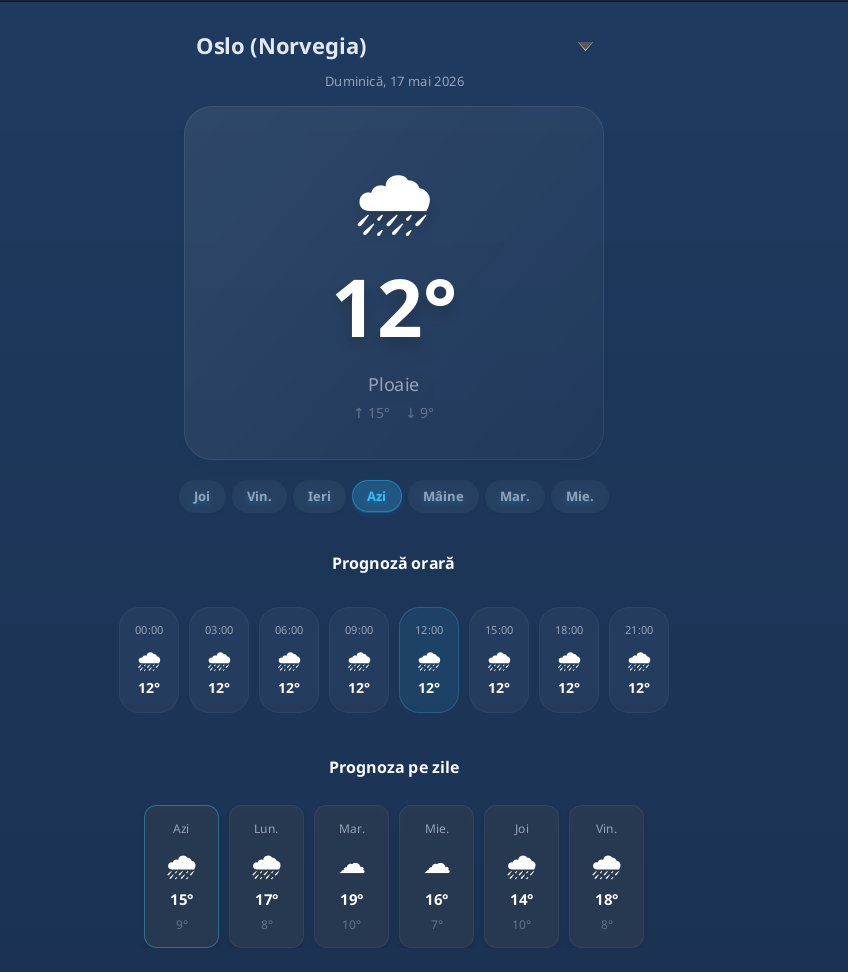
\includegraphics[width=0.60\textwidth]{screenshots/vremea_oras_prognoza.png}
\caption{Tab-ul ``Acum" --- Dashboard unificat (prognoza 10 zile, probabilitati, clasamente, anomalii)}
\label{fig:tab_acum}
\end{figure}

\begin{figure}[H]
\centering
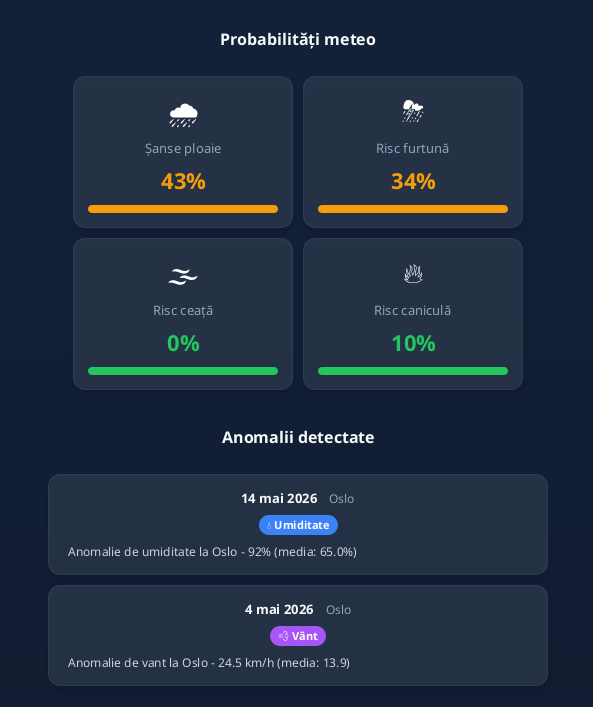
\includegraphics[width=0.60\textwidth]{screenshots/probabilitati_anomalii.png}
\caption{Carduri de probabilitati meteo si anomalii detectate}
\label{fig:prob_cards}
\end{figure}

\begin{figure}[H]
\centering
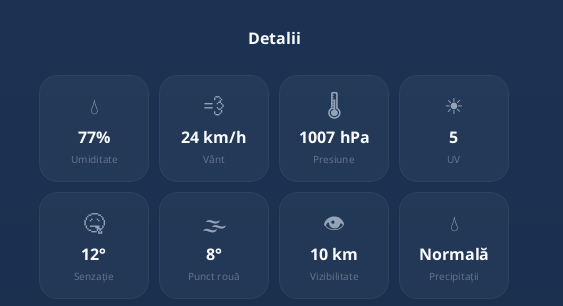
\includegraphics[width=0.60\textwidth]{screenshots/detalii.png}
\caption{Detalii meteorologice --- umiditate, vant, UV, presiune, punct de roua}
\label{fig:detalii}
\end{figure}

\subsection{Tab-ul ``Harta"}

O harta interactiva a Europei desenata pe canvas JavaFX (1200$\times$800 px) cu 40 de poligoane de tari colorate in functie de temperatura medie (pseudo-relief). Orasele majore afiseaza badge-uri cu temperaturi min/max. Harta include: zoom in/out (0.5$\times$--3.0$\times$), panning prin drag, selector de data si buton Play care animeaza automat evolutia vremii de la data selectata pana la ziua curenta, cadru cu cadru.

\begin{figure}[H]
\centering
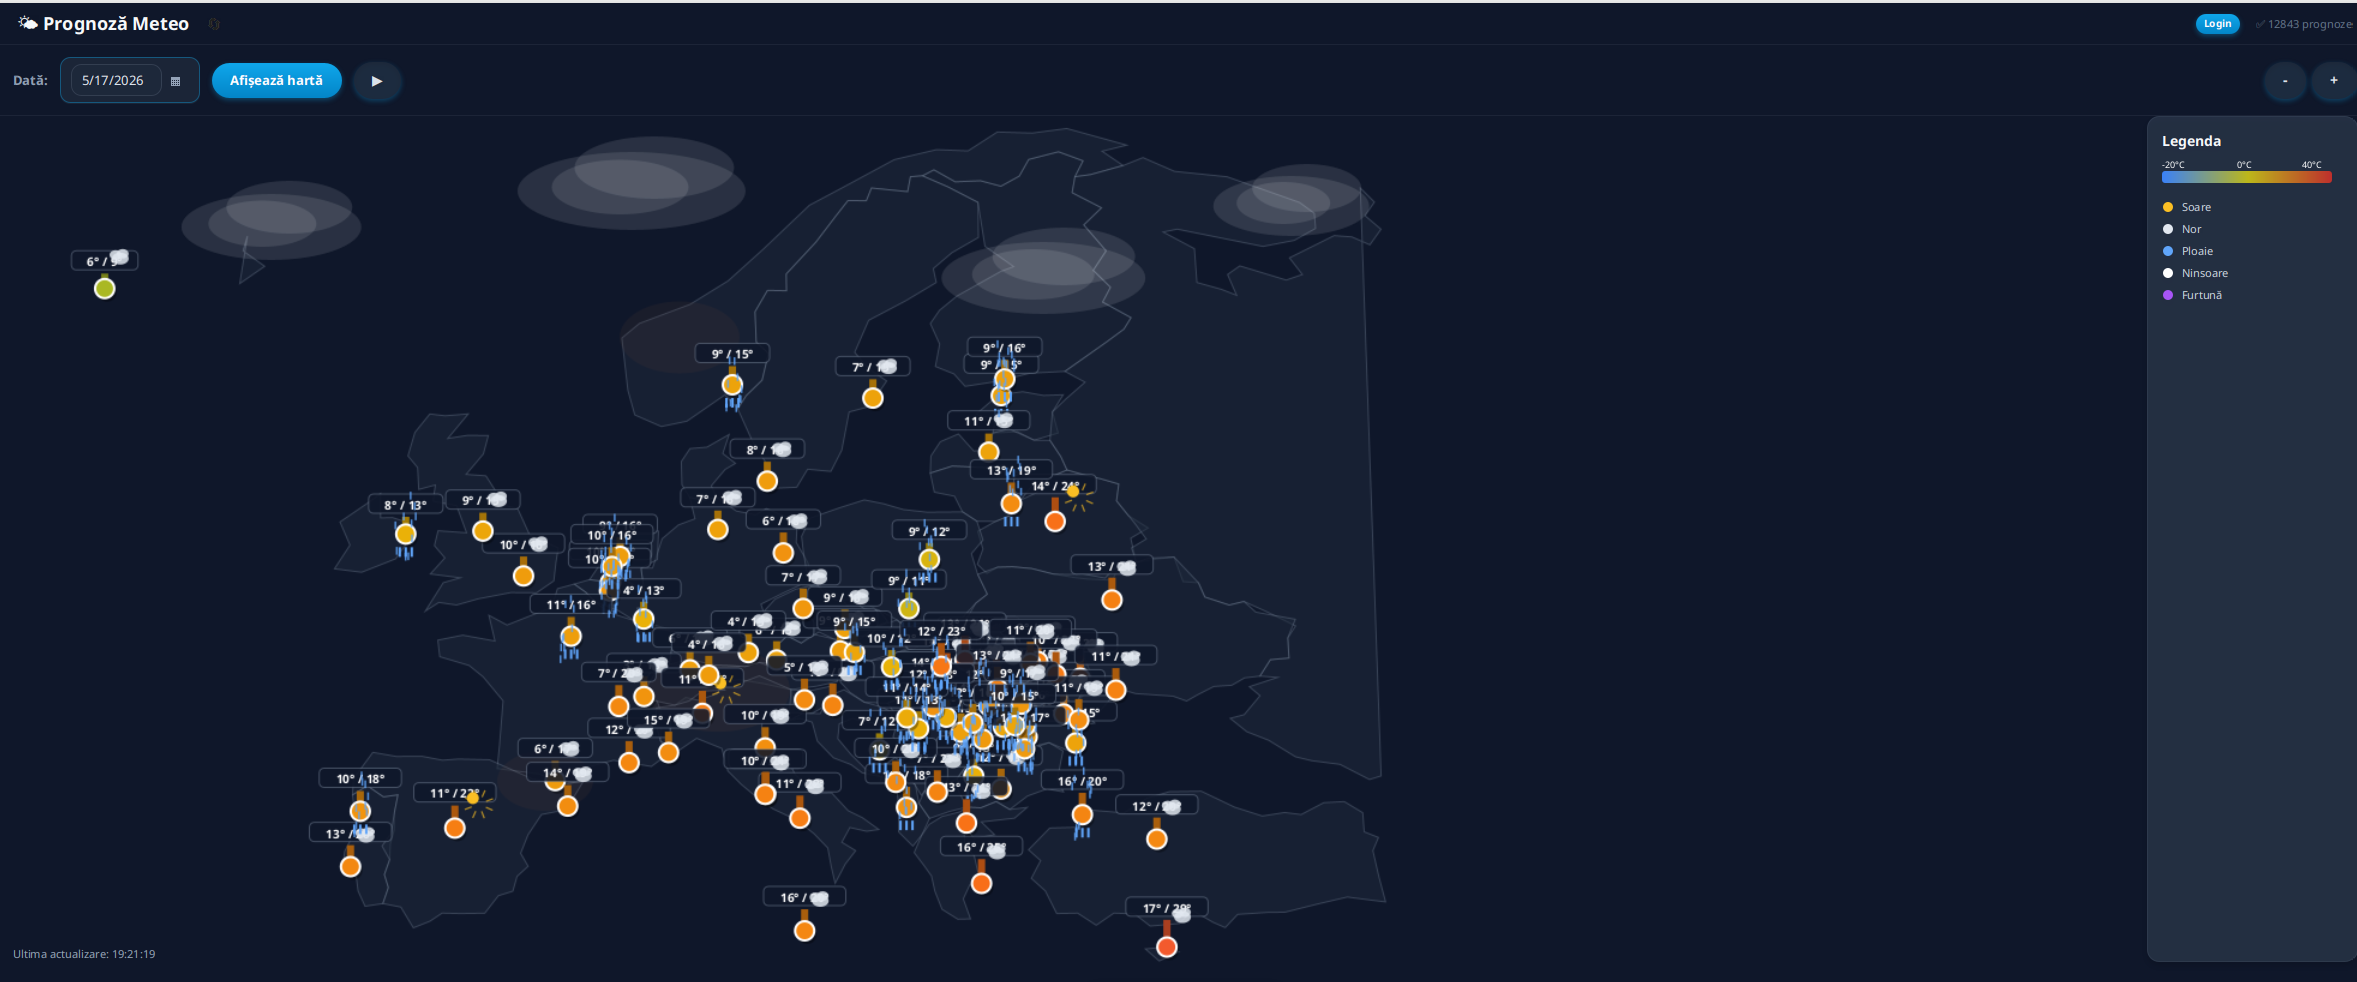
\includegraphics[width=0.60\textwidth]{screenshots/harta.png}
\caption{Tab-ul ``Harta" --- Europa 40 tari, 93 orase, zoom/pan, play evolutie}
\label{fig:tab_harta}
\end{figure}

\subsection{Tab-ul ``Mai multe"}

Contine autentificare reala cu verificare in baza de date (tabela \texttt{users}, parola criptata SHA-256), setari (unitati de temperatura, unitati de vant, sincronizare automata), sectiunea de comunitate (comentarii si voturi) si informatii despre aplicatie.\newline\indent\textbf{User de test}: \texttt{username=user}, \texttt{password=user}.

\begin{figure}[H]
\centering
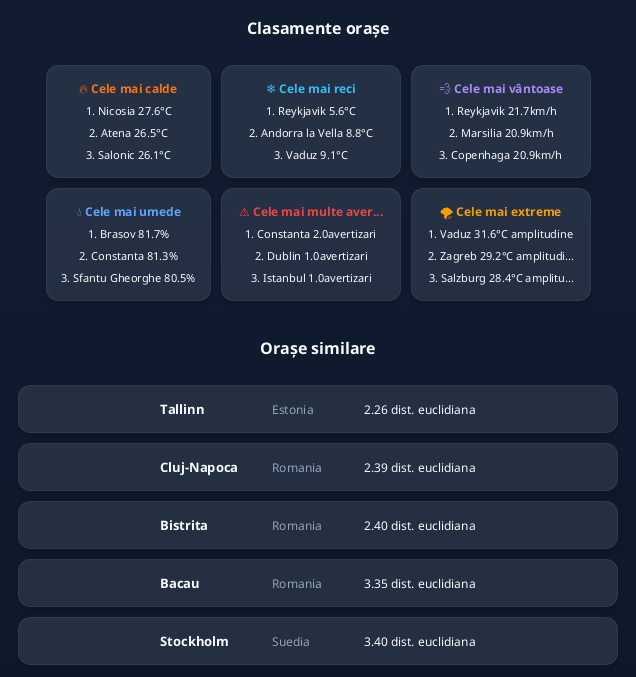
\includegraphics[width=0.60\textwidth]{screenshots/orase_clasamente_similare.png}
\caption{Clasamente orase si orase similare}
\label{fig:clasamente}
\end{figure}

\vspace{0.8cm}

% ========== 7. ALGORITMI COMPLECSI PE SERVER ==========
\section{Algoritmi complexi implementati in PL/pgSQL}

Aceasta sectiune prezinta in detaliu algoritmii non-triviali implementati la nivelul serverului PostgreSQL. Acestia reprezinta nucleul valorii adaugate a proiectului si justifica punctajul maxim pentru complexitate.

\subsection{Algoritmi de Machine Learning --- Prezentare generala}

Algoritmii de Machine Learning ruleaza in 7 etape, toate implementate ca proceduri stocate:

\begin{algobox}[Algoritmi de Machine Learning end-to-end]
\begin{enumerate}
    \item \texttt{sp\_build\_weather\_vector}: construieste vectori 25D din datele brute;
    \item \texttt{sp\_compute\_recipe\_scores}: aplica detectoare fuzzy pentru 6 fenomene meteo;
    \item \texttt{sp\_label\_regimes}: clasifica regimurile pe baza centroidelor;
    \item \texttt{sp\_build\_markov\_tensor}: construieste tensorul de tranzitii de ordin 2;
    \item \texttt{sp\_run\_monte\_carlo}: simuleaza 5000 de traiectorii;
    \item \texttt{sp\_detect\_anomalies}: identifica deviatii statistice ($2\sigma$);
    \item \texttt{sp\_forecast\_score}: calculeaza scorul ponderat al prognozelor.
\end{enumerate}
\end{algobox}

\subsection{Vectorizarea meteo --- \texttt{sp\_build\_weather\_vector}}

Procedura transforma datele brute din \texttt{forecasts} intr-un vector de 25 de dimensiuni care captureaza starea meteorologica a unei zile. Fiecare dimensiune reprezinta un feature inginerit:

\begin{align*}
v = [&\text{temp\_min}, \text{ temp\_max}, \text{ temp\_mean}, \text{ temp\_range}, \\
    &\text{wind\_speed}, \text{ wind\_gust\_proxy}, \text{ humidity}, \\
    &\text{uv\_index}, \text{ uv\_level}, \text{ precip\_sum}, \\
    &\text{precip\_hours}, \text{ pressure}, \text{ sunshine}, \\
    &\text{dew\_point}, \text{ cloud\_cover\_proxy}, \dots]
\end{align*}

Algoritmul utilizeaza un \textbf{cursor} care itereaza cronologic prin prognozele unui oras si calculeaza derivate temporale (diferente fata de $t-1$ si $t-2$). Aceste derivate captureaza tendinte: o crestere brusca a temperaturii sau a presiunii este un indicator predictiv important.

\begin{lstlisting}[caption={Fragment din vectorizare --- calculul derivatelor temporale}]
-- Delta fata de ziua anterioara
v[16] := COALESCE(curr.temp_max - prev1.temp_max, 0);
v[17] := COALESCE(curr.temp_min - prev1.temp_min, 0);
v[18] := COALESCE(curr.wind_speed - prev1.wind_speed, 0);

-- A doua derivata (acceleratie)
v[19] := COALESCE((curr.temp_max - prev1.temp_max)
    - (prev1.temp_max - prev2.temp_max), 0);
\end{lstlisting}

\textbf{De ce este complex?} Constructia vectorului necesita accesul la fereastra temporala $[t-2, t]$ pentru fiecare zi, ceea ce implica auto-join-uri sau gestiune de cursor cu variabile de stare. Vectorul final este stocat ca array PostgreSQL \texttt{DOUBLE PRECISION[]} pentru eficienta.

\subsection{Inferenta fuzzy --- \texttt{sp\_compute\_recipe\_scores}}

Aceasta procedura implementeaza un \textbf{sistem de inferenta fuzzy} cu 6 detectoare de fenomene meteorologice. Fiecare detector combina mai multi parametri prin functii de apartenenta (sigmoide si gaussiene).

\subsubsection{Functii de apartenenta}

\begin{lstlisting}[caption={Functii fuzzy implementate ca functii PostgreSQL}]
CREATE OR REPLACE FUNCTION fn_sigmoid(x DOUBLE PRECISION,
    center DOUBLE PRECISION, slope DOUBLE PRECISION)
RETURNS DOUBLE PRECISION AS $$
BEGIN
    RETURN 1.0 / (1.0 + EXP(-slope * (x - center)));
END;
$$ LANGUAGE plpgsql IMMUTABLE;

CREATE OR REPLACE FUNCTION fn_rev_sigmoid(x DOUBLE PRECISION,
    center DOUBLE PRECISION, slope DOUBLE PRECISION)
RETURNS DOUBLE PRECISION AS $$
BEGIN
    RETURN 1.0 / (1.0 + EXP(slope * (x - center)));
END;
$$ LANGUAGE plpgsql IMMUTABLE;
\end{lstlisting}

\subsubsection{Detectorul de canicula}

\begin{align*}
\mu_{\text{caldura}} &= \sigma^+(T_{\text{max}}, 30, 0.3) \\
\mu_{\text{umiditate}} &= \sigma^-(H, 40, 0.08) \\
\mu_{\text{presiune}} &= \sigma^-(P, 1013, 0.02) \\
\text{score}_{\text{canicula}} &= \min(\mu_{\text{caldura}}, \mu_{\text{umiditate}}, \mu_{\text{presiune}}) \times w_{\text{sezon}}
\end{align*}

unde $\sigma^+$ este sigmoida directa, $\sigma^-$ este sigmoida inversa, iar $w_{\text{sezon}}$ este un multiplicator sezonier (vara = 1.5, iarna = 0.3).

\textbf{De ce este complex?} Fiecare detector combina 3--5 variabile meteorologice prin operatori fuzzy AND (implementati cu \texttt{LEAST}). Scoarele finale sunt stocate ca JSONB pentru flexibilitate.

\subsection{Lanturi Markov de ordin 2 --- \texttt{sp\_build\_markov\_tensor}}

Procedura construieste un \textbf{tensor de tranzitii de ordin 2}:

\begin{equation}
P(R_{t+1} = r_{next} \mid R_t = r_{curr}, R_{t-1} = r_{prev})
\end{equation}

\begin{lstlisting}[caption={Constructia tensorului Markov de ordin 2}]
INSERT INTO markov_transitions (climate_zone, season, r_prev, r_curr, r_next, probability)
SELECT
    dr.climate_zone,
    fn_get_season(dr.forecast_date) AS season,
    LAG(dr.regime_id, 1) OVER w AS r_prev,
    dr.regime_id AS r_curr,
    LEAD(dr.regime_id, 1) OVER w AS r_next,
    COUNT(*)::DOUBLE PRECISION / SUM(COUNT(*)) OVER (
        PARTITION BY dr.climate_zone, fn_get_season(dr.forecast_date),
                     LAG(dr.regime_id, 1) OVER w, dr.regime_id
    ) AS probability
FROM daily_regimes dr
WINDOW w AS (PARTITION BY dr.city_id ORDER BY dr.forecast_date)
HAVING LAG(dr.regime_id, 1) OVER w IS NOT NULL
   AND LEAD(dr.regime_id, 1) OVER w IS NOT NULL;
\end{lstlisting}

\textbf{Explicatie algoritmica}:
\begin{enumerate}
    \item Fereastra \texttt{WINDOW w} defineste o partitie pe oras ordonata cronologic;
    \item \texttt{LAG(regime\_id, 1)} extrage regimul la $t-1$;
    \item \texttt{LEAD(regime\_id, 1)} extrage regimul la $t+1$;
    \item Probabilitatea este normalizata per grup $(\text{climate\_zone}, \text{season}, r_{prev}, r_{curr})$;
    \item Rezultatul este un tensor 4D conditionat de zona climatica si sezon.
\end{enumerate}

\textbf{De ce este complex?} Spre deosebire de un lant Markov clasic (ordin 1), modelul de ordin 2 captureaza dependente pe 3 zile consecutive. Acest lucru permite predictii mai precise pentru fenomene cu persistenta (ex. val de caldura care dureaza 3--4 zile).

\subsection{Modelul Markov Ascuns (HMM) --- \texttt{fn\_update\_hmm\_emission}}

Procedura implementeaza pasul M (Maximization) al algoritmului \textbf{Baum-Welch} pentru un HMM discret cu $N = 4$ stari ascunse si $M = 16$ simboli observabili (regimurile).

\begin{lstlisting}[caption={Normalizarea probabilitatilor de emisie in HMM}]
CREATE OR REPLACE FUNCTION fn_update_hmm_emission(
    city_id INTEGER, state_id INTEGER, new_probs DOUBLE PRECISION[]
)
RETURNS VOID AS $$
DECLARE
    clamped DOUBLE PRECISION[];
    total DOUBLE PRECISION := 0.0;
    i INTEGER;
BEGIN
    -- Clamp la [0.01, 0.99]
    FOR i IN 1..16 LOOP
        clamped[i] := GREATEST(0.01, LEAST(0.99, COALESCE(new_probs[i], 0.0625)));
        total := total + clamped[i];
    END LOOP;

    -- Renormalizare iterativa pentru suma = 1.0
    FOR i IN 1..16 LOOP
        clamped[i] := clamped[i] / total;
    END LOOP;

    UPDATE hidden_states
    SET emission_probs = clamped
    WHERE city_id = $1 AND state_id = $2;
END;
$$ LANGUAGE plpgsql;
\end{lstlisting}

\textbf{De ce este complex?}
\begin{itemize}
    \item Manipularea de array-uri 1-indexate in PL/pgSQL necesita atentie la limite;
    \item Clamping-ul previne probabilitati de 0 sau 1 (care ar anula anumite traiectorii in forward-backward);
    \item Renormalizarea iterativa garanteaza ca suma probabilitatilor de emisie este exact 1.0, respectand axiomele probabilitatii.
\end{itemize}

\subsection{Simulare Monte Carlo --- \texttt{sp\_run\_monte\_carlo}}

Aceasta este cea mai sofisticata procedura. Ea genereaza 5000 de traiectorii meteorologice pentru urmatoarele 10 zile.

\subsubsection{Algoritmul de esantionare a regimului urmator}

Pentru fiecare zi $d$ si fiecare traiectorie $i$:
\begin{enumerate}
    \item Se identifica regimurile anterioare $(r_{d-2}, r_{d-1})$;
    \item Se cauta in tensorul Markov toate tranzitiile posibile $r_{next}$ si probabilitatile asociate;
    \item Se genereaza un numar aleator $u \sim U(0,1)$;
    \item Se parcurge lista cumulativa de probabilitati pana cand suma depaseste $u$ (\textbf{cumulative probability walk}):
    \begin{equation}
    r_d = \min \left\{ r \mid \sum_{k=1}^{r} P(R_k \mid r_{d-2}, r_{d-1}) \geq u \right\}
    \end{equation}
\end{enumerate}

\subsubsection{Generarea temperaturii conditionate de regim}

Dupa ce regimul $r_d$ este esantionat, temperatura este generata prin:
\begin{equation}
T_d = \mu_{\text{clim}}(doy) + \epsilon, \quad \epsilon \sim \mathcal{N}(0, \sigma_{\text{regim}})
\end{equation}
unde $\mu_{\text{clim}}(doy)$ este media climatologica pentru ziua din an (doy), extrasa din \texttt{seasonal\_climatology}, iar $\sigma_{\text{regim}}$ este deviatia standard asociata regimului $r_d$.

\subsubsection{Extragerea percentilelor}

Dupa simularea tuturor traiectoriilor, se calculeaza:
\begin{align*}
\text{P10} &= Q_{0.10}(\{T_d^{(i)}\}_{i=1}^{5000}) \\
\text{P50} &= Q_{0.50}(\{T_d^{(i)}\}_{i=1}^{5000}) = \text{mediana} \\
\text{P90} &= Q_{0.90}(\{T_d^{(i)}\}_{i=1}^{5000})
\end{align*}

Aceste benzi de incredere sunt salvate in \texttt{monte\_carlo\_predictions} si afisate in JavaFX ca grafic cu 3 benzi.

\begin{figure}[H]
\centering
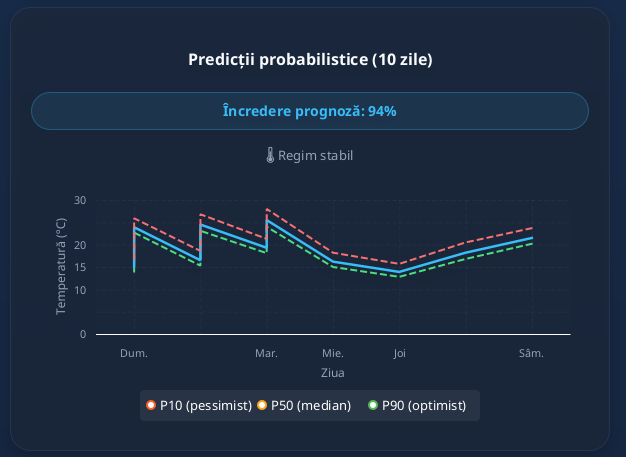
\includegraphics[width=0.60\textwidth]{screenshots/predictii_probabilistice.png}
\caption{Predictii probabilistice --- benzile P10/P50/P90}
\label{fig:pred_prob}
\end{figure}

\begin{figure}[H]
\centering
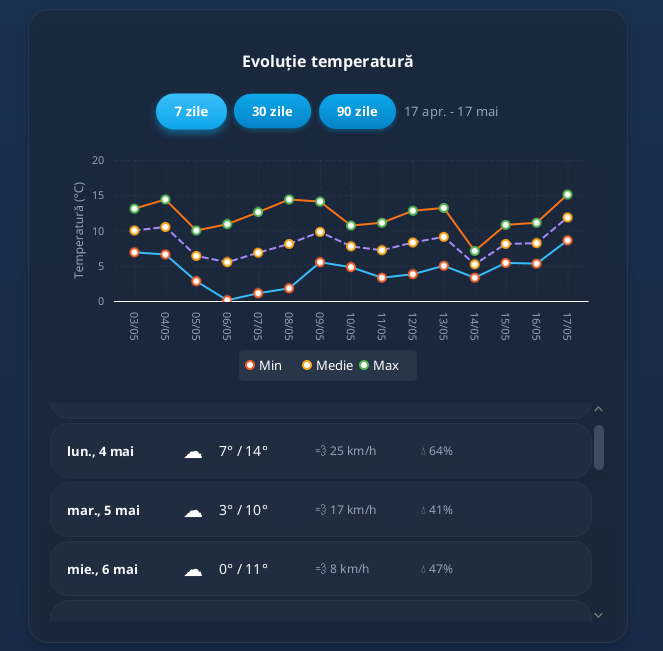
\includegraphics[width=0.60\textwidth]{screenshots/evolutie_temperatura.png}
\caption{Evolutia temperaturii pe 30 de zile}
\label{fig:evolutie}
\end{figure}

\begin{figure}[H]
\centering
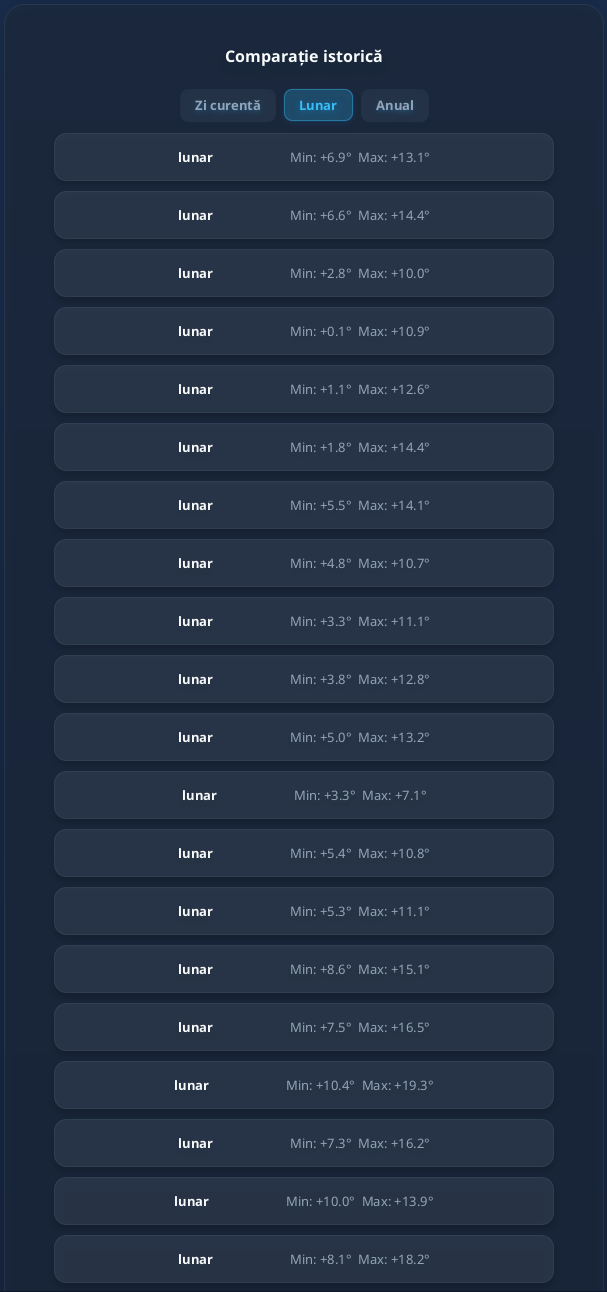
\includegraphics[width=0.60\textwidth]{screenshots/comparatie_istorica.png}
\caption{Comparatie istorica --- diferente fata de mediile climatologice}
\label{fig:comparatie}
\end{figure}

\subsection{Detectia anomaliilor --- \texttt{sp\_detect\_anomalies}}

Procedura implementeaza o metoda statistica clasica: \textbf{regula celor $2\sigma$}.

\begin{lstlisting}[caption={Identificarea anomaliilor prin deviatia standard}]
SELECT f.city_id, f.date, f.temp_max,
       stats.avg_temp, stats.stddev_temp,
       (f.temp_max - stats.avg_temp) / NULLIF(stats.stddev_temp, 0) AS z_score
FROM forecasts f
CROSS JOIN LATERAL (
    SELECT AVG(f2.temp_max) AS avg_temp,
           STDDEV(f2.temp_max) AS stddev_temp
    FROM forecasts f2
    WHERE f2.city_id = f.city_id
      AND EXTRACT(MONTH FROM f2.date) = EXTRACT(MONTH FROM f.date)
) stats
WHERE ABS(f.temp_max - stats.avg_temp) > 2 * stats.stddev_temp;
\end{lstlisting}

\textbf{Explicatie}:
\begin{itemize}
    \item Subcererea \texttt{LATERAL} calculeaza media si deviatia standard pentru fiecare luna, per oras;
    \item O prognoza este marcata ca anomalie daca deviaza cu mai mult de $2\sigma$ de la media sezoniera;
    \item Acelasi calcul se aplica pentru vant, umiditate si UV.
\end{itemize}

\textbf{De ce este complex?} Utilizarea \texttt{LATERAL} permite corelarea subcererii cu randul exterior fara a repeta codul. Aceasta este o tehnica avansata de optimizare in PostgreSQL.

\subsection{Clasificarea oraselor similare --- \texttt{sp\_classify\_similar\_cities}}

Procedura calculeaza distanta euclidiana in 4 dimensiuni intre profilul unui oras de referinta si toate celelalte orase:

\begin{equation}
d(o_{ref}, o_i) = \sqrt{(T_{min}^{ref} - T_{min}^{i})^2 + (T_{max}^{ref} - T_{max}^{i})^2 + (H^{ref} - H^{i})^2 + (W^{ref} - W^{i})^2}
\end{equation}

Rezultatele sunt ordonate crescator si returnate ca lista de orase similare.

\subsection{Scorul prognozelor si reputatia}

\subsubsection{Scorul unei prognoze --- \texttt{sp\_forecast\_score}}

\begin{equation}
\text{score}(f) = \frac{\sum_{v \in V_f} w(v) \cdot \mathbb{I}(v.\text{is\_accurate})}{\sum_{v \in V_f} w(v)}, \quad w(v) = 1 + \ln(1 + \text{reputation}(v.\text{user}))
\end{equation}

Voturile utilizatorilor cu reputatie mai mare au pondere mai mare, dar cresterea este logaritmica pentru a preveni dominarea de catre ``super-utilizatori".

\subsubsection{Reputatia utilizatorilor --- \texttt{sp\_user\_reputation}}

\begin{equation}
\text{reputation}(u) = \text{avg\_accuracy}(u) \times \ln(1 + \text{comment\_count}(u) + 1)
\end{equation}

Factorul logaritmic $\ln(1 + n + 1)$ recompenseaza participarea activa (comentarii), dar cu diminuarea returnarilor --- primul comentariu aduce cel mai mult, al zecelea aduce mai putin.

\vspace{0.8cm}

% ========== 8. TESTARE SI VALIDARE ==========
\section{Testare si validare}

Proiectul include un set comprehensiv de teste unitare si de integrare:

\begin{table}[H]
\centering
\begin{tabular}{@{}llcc@{}}
\toprule
\textbf{Clasa de test} & \textbf{Scop} & \textbf{Teste} & \textbf{Status} \\
\midrule
\texttt{CityServiceTest} & Servicii orase/tari & 5 & Pass \\
\texttt{ForecastServiceTest} & Prognoze, comparatii & 4 & Pass \\
\texttt{StatisticsServiceTest} & Statistici, clasamente & 3 & Pass \\
\texttt{UserServiceTest} & Voturi, comentarii & 3 & Pass \\
\texttt{AccuracyServiceTest} & Scoruri, reputatie & 2 & Pass \\
\texttt{SessionManagerTest} & Management sesiune & 3 & Pass \\
\texttt{DatabaseConnectionPoolTest} & Pool HikariCP & 3 & Pass \\
\texttt{DatabaseInitializerTest} & Migrari DB & 3 & Pass \\
\texttt{ClusteringServiceTest} & K-means, silhouette & 9 & Pass \\
\texttt{HmmTrainingServiceTest} & Forward-backward, Baum-Welch & 5 & Pass \\
\texttt{MlPipelineIntegrationTest} & Flux end-to-end & 1 & Pass \\
\midrule
\textbf{TOTAL} & & \textbf{63} & \textbf{63 Pass} \\
\bottomrule
\end{tabular}
\caption{Rezultate teste}
\end{table}

Testul de integrare \texttt{MlPipelineIntegrationTest} valideaza intregul flux de algoritmi de Machine Learning cu date reale de la Open-Meteo pentru Bucuresti: importa 365 de zile istorice, construieste vectori, ruleaza clustering, Markov, HMM si Monte Carlo, apoi verifica consistenta percentilelor ($\text{P10} \leq \text{P50} \leq \text{P90}$) si faptul ca toate probabilitatile sunt in $[0, 1]$.

% ========== 9. BIBLIOGRAFIE ==========
\section{Bibliografie}

\begin{thebibliography}{9}

\bibitem{markov_weather} Rabiner, L. R. (1989). ``A tutorial on hidden Markov models and selected applications in speech recognition." \textit{Proceedings of the IEEE}, 77(2), 257--286. Aplicatia extinde HMM-urile pentru modelarea regimurilor meteorologice, folosind algoritmul Baum-Welch pentru estimarea parametrilor.

\bibitem{markov_chains} Norris, J. R. (1998). \textit{Markov Chains}. Cambridge University Press. Lanturile Markov de ordin 2 implementate in \texttt{sp\_build\_markov\_tensor} permit capturarea persistentei fenomenelor meteorologice pe 3 zile consecutive, spre deosebire de modelele de ordin 1.

\bibitem{monte_carlo} Robert, C. P., \& Casella, G. (2004). \textit{Monte Carlo Statistical Methods}. Springer. Simularea cu 5000 de traiectorii si extragerea percentilelor (P10, P50, P90) urmeaza metodologia clasica a estimarii distributiilor predictive prin resampling.

\bibitem{fuzzy_logic} Ross, T. J. (2010). \textit{Fuzzy Logic with Engineering Applications}. Wiley. Detectoarele fuzzy (canicula, furtuna, ceata) din \texttt{sp\_compute\_recipe\_scores} folosesc functii de apartenenta sigmoidale si operatori T-norm (\texttt{LEAST}) conform teoriei sistemelor fuzzy.

\bibitem{postgres_docs} The PostgreSQL Global Development Group. \textit{PostgreSQL 16 Documentation} --- \url{https://www.postgresql.org/docs/16/}. Procedurile stocate PL/pgSQL, functiile de fereastra (\texttt{LAG}, \texttt{LEAD}), tipurile array si JSONB sunt documentate oficial.

\bibitem{open_meteo} Zippenfenig, P. (2023). ``Open-Meteo.com Weather API." \url{https://open-meteo.com/}. Sursa gratuita de date meteorologice istorice si de prognoza, utilizata pentru popularea automata a tabelei \texttt{forecasts}.

\bibitem{db_design} Elmasri, R., \& Navathe, S. B. (2015). \textit{Fundamentals of Database Systems}. Pearson. Capitolele privind normalizarea (3NF, BCNF) si proiectarea diagramelor E/A au constituit baza teoretica a schemei bazei de date.

\bibitem{jdbc} Oracle Corporation. \textit{The Java Tutorials --- JDBC Basics}. \url{https://docs.oracle.com/javase/tutorial/jdbc/}. Conectivitatea JDBC directa (fara ORM) a fost aleasa pentru a demonstra controlul explicit al transactiilor si al apelurilor de proceduri stocate.

\bibitem{hikari} brettwooldridge. \textit{HikariCP}. \url{https://github.com/brettwooldridge/HikariCP}. Pool-ul de conexiuni HikariCP gestioneaza eficient conexiunile TCP catre PostgreSQL, reducand overhead-ul de initializare la fiecare query.

\bibitem{kmeans} Arthur, D., \& Vassilvitskii, S. (2007). ``k-means++: The advantages of careful seeding." \textit{SODA '07}. Clustering-ul regimurilor meteorologice foloseste k-means++ prin Apache Commons Math pentru initializarea centroidelor.

\end{thebibliography}

\newpage

% ========== 10. CONCLUZII ==========
\section{Concluzii}

Prezentul proiect demonstreaza ca un sistem de gestiune a bazelor de date relationale (PostgreSQL) poate gazdui nu doar operatii CRUD, ci si algoritmi sofisticati de machine learning si simulare statistica. Prin transferarea algoritmilor de predictie la nivelul serverului, am obtinut:

\begin{itemize}
    \item \textbf{Coerenta tranzactionala}: actualizarile datelor si ale modelului sunt atomice;
    \item \textbf{Performanta}: eliminarea transferului de date masive intre server si client;
    \item \textbf{Auditabilitate}: fiecare parametru al modelului este istorisit in tabele relationale.
\end{itemize}

Schema bazei de date, proiectata in \textbf{BCNF}, extinde modelul clasic entitate-relatie cu tabele specializate pentru vectori, regimuri, tranzitii Markov, stari HMM si predictii Monte Carlo. Toate tabelele sunt populate automat prin scripturi de migrare si import de la API-ul Open-Meteo.

\textbf{Directii viitoare}:
\begin{enumerate}
    \item Implementarea unui model HSMM (Hidden Semi-Markov Model) pentru capturarea duratei regimurilor;
    \item Parallelizarea simularii Monte Carlo cu \texttt{pg\_parallel};
    \item Integrarea cu modelul de limbaj pentru generarea de rapoarte meteo in limbaj natural.
\end{enumerate}

\vfill
\begin{center}
\rule{0.5\textwidth}{0.4pt}\\[0.3cm]
\textit{Negura Alexandru Teodor}\\
\textit{Facultatea de Informatica, UAIC Iasi}\\
\textit{Anul universitar 2025--2026}
\end{center}

\end{document}
